%%%%%%%%%%%%%%%%%%%%%%%%%%%%%%%%%%%%%%%%%%%%%%%%%%%%%%%%%%%%%%%%%%%%%%%%%%%%%%%%
%%% Results
%%%%%%%%%%%%%%%%%%%%%%%%%%%%%%%%%%%%%%%%%%%%%%%%%%%%%%%%%%%%%%%%%%%%%%%%%%%%%%%%

\clearpage
\section{Discussion}
\label{sec:discussion}

In this section I will describe the results of my research and development.
I will first describe the final product of my development.
Then I will list the numerical data from the machine learning experiments.
\nyi{User satisfaction}
Lastly I will examine the answers for the research questions and
evaluate the value of the thesis.

\subsection{Results}

%T\"ass\"a osassa esitet\"a\"an tulokset ja vastataan tutkielman alussa
%esitettyihin tutkimuskysymyksiin. Tieteellisen kirjoitelman
%arvo mitataan t\"ass\"a osassa esitettyjen tulosten perusteella.

\begin{figure}[htb]
\centering 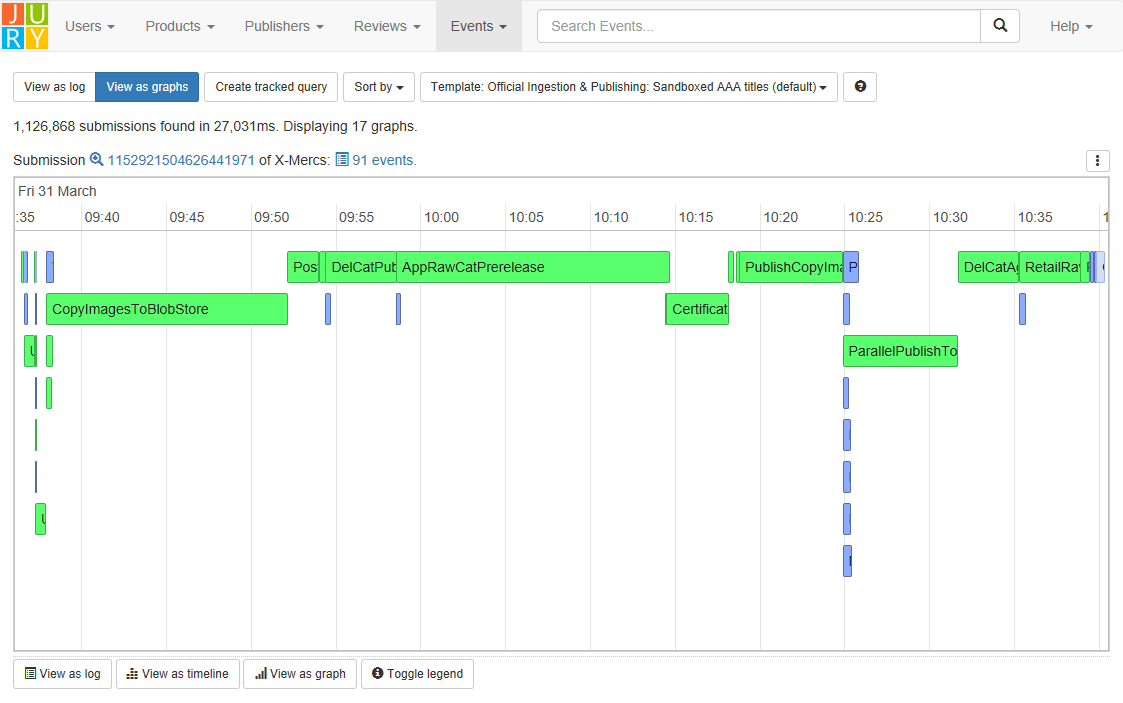
\includegraphics[width=\linewidth]{gfx/timeline.png}
\caption{Timeline view \label{fig:timeline}}
\end{figure}

\begin{figure}[htb]
\centering 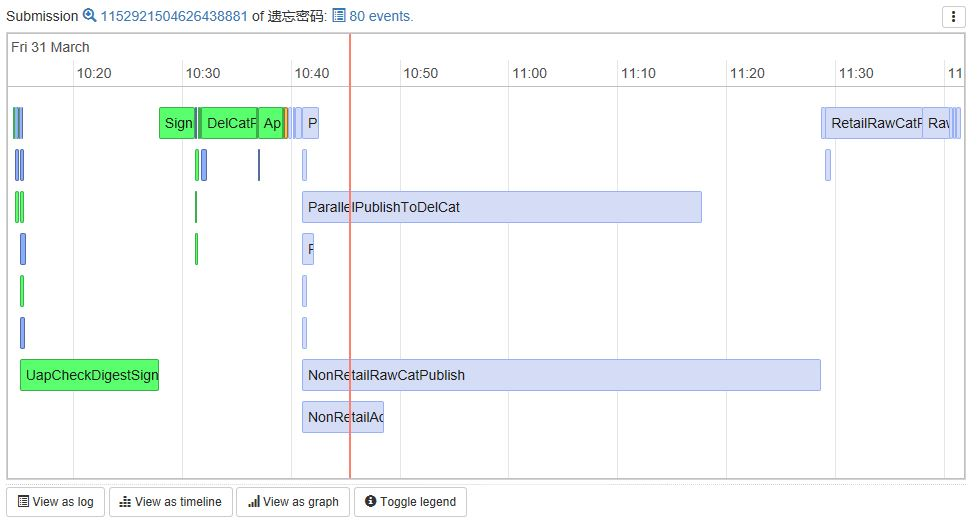
\includegraphics[width=\linewidth]{gfx/estimates.jpg}
\caption{Timeline view with estimates \label{fig:estimates}}
\end{figure}

\begin{figure}[htb]
\centering 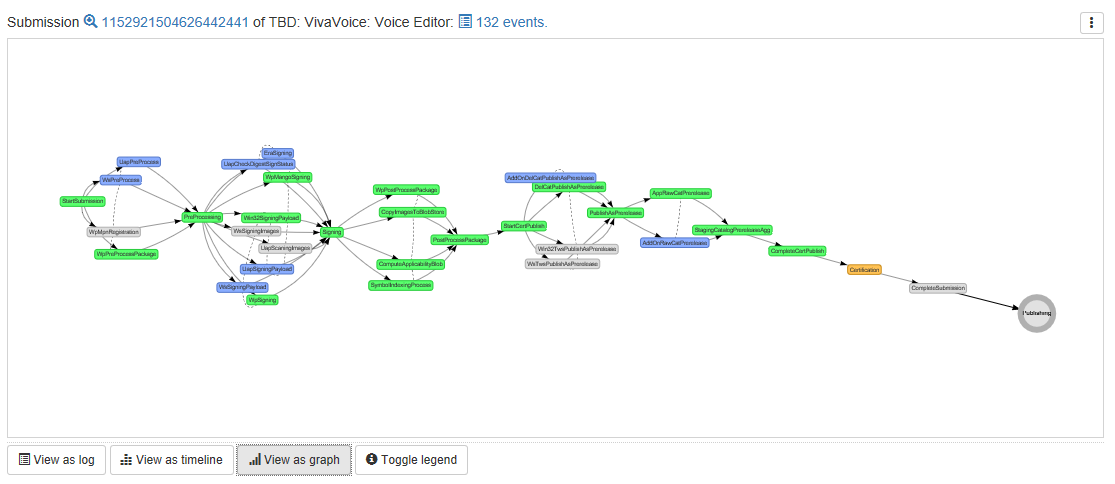
\includegraphics[width=\linewidth]{gfx/graph.png}
\caption{Graph view \label{fig:graph}}
\end{figure}

Figure \ref{fig:timeline} shows the final product developed in this thesis.
The topmost bar is the main navigation of the website.
On the navigation bar the user can query the events.
The page below can display any number of traces corresponding to the events that match the user's query.
If a large number of traces would be returned, the view is paged.
The second bar under the navigation is the event navigation bar I developed, which includes all the functionality that affects all the content on the vents page.
It allows the user to switch between the log view (See figure \ref{fig:plaineventlog}) and the visualizations.
It also includes functionality for sorting the visualizations and choosing which process model to build the visualization from.

Each trace returned by the query is visualized as a timeline or a graph. On top of the visualization the user can see the basic information about the trace containing the submission ID and the name of the product.
Under the visualization there are options to choose how the visualization is displayed (between the log view, the graph view, and the timeline view) and an option to toggle help.
The visualization can be manipulated with the mouse or a touch screen. It allows panning and zooming actions.
The user can select or mouseover individual events to see all the metadata related to the event.

In the timeline view (figure \ref{fig:timeline}) the visualization is set on top of a horizontal axis that corresponds to time. The activities shown have start and end times which can be seen visually or in the metadata.
Parallel activities are stacked on top of each other.
Figure \ref{fig:estimates} shows the estimations for an incomplete submission.
The activities yet to happen are drawn with a faint blue color and their estimated start and end times are visualized similarly as the logged activities.
The red line describes the current time.
The user can visually see the status of the submission and the activities that are predicted to have happened already.

Figure \ref{fig:graph} shows the alternate directed graph view. In the graph view the directed graph is drawn for the user. The graph nodes are interactive and the edges act as two-dimensional springs.
The user can thus manipulate the nodes and move them. Panning and zooming actions are also enabled.

\nyi{Talk about user satisfaction here?}

\begin{table}[htb]
\begin{center}
\begin{tabularx}{\linewidth}{| X | r | r |}
\hline
Dataset & Mean Absolute Error & RMSE \\
\hline
\textbf{TP50 value (median)} &  & \\
JSON template                       & 573.3 & 5871.4 \\
Automatically generated template    & 919.6 & 9937.3 \\
\hline
\textbf{TP75 value} &  & \\
JSON template                       & 710.5 & 5484.2 \\
Automatically generated template    & 954.0 & 9904.8 \\
\hline
\end{tabularx}
\end{center}
\caption{Results from plain statistics}
\label{tab:statresults}
\end{table}

To evaluate the results of the machine learning models, I first calculated a baseline for comparison.
The baseline consists of the same simple statistics as were used for the estimates in the application, the TP50 (median) and the TP75.
I calculated these two values for each transition (graph edge) based on the training set to construct a simple model. 
In the model each transition corresponds to a single value (the TP50 or the TP75). 
When predicting, the model always returns this value based on the transition in question.
Table \ref{tab:statresults} lists the results from this baseline model. 
The values of \textit{mean absolute error} and \textit{root mean square error} are listed.

I used the same training and testing sets to find the same error values for each machine learning model.
The error values are listed in table \ref{tab:mlresults}.

\begin{table}[htb]
\begin{center}
\begin{tabularx}{\linewidth}{| X | r | r | r | r |}
\hline
~ & \multicolumn{2}{c|}{BDT} & \multicolumn{2}{c|}{Poisson} \\
Dataset & Absolute & RMSE & Absolute & RMSE \\
\hline
\textbf{JSON template} &  &  &  &  \\
No extra features                   & 809.1 & 6290.7 & 881.1 & 5970.6 \\
with current time                   & 825.2 & 6130.3 & 881.1 & 5971.0 \\
with manual review                  & 689.7 & 5819.0 & 809.3 & 5800.9 \\
with resubmission                   & 831.5 & 6255.3 & 881.1 & 5971.2 \\
with manual review and resubmission & 703.7 & 5807.5 & 808.9 & 5800.8 \\
with all extra features             & 693.5 & 5801.9 & 808.3 & 5800.4 \\
\hline
\textbf{Automatically generated template} &  &  &  &  \\
No extra features                   & 994.8 & 5756.3 & 1243.9 & 6563.3 \\
with current time                   & 1099.7 & 6470.5 & 1225.8 & 6558.7 \\
with manual review                  & 815.1 & 5332.1 & 1038.5 & 5785.0 \\
with resubmission                   & 1004.3 & 5845.3 & 1219.1 & 6553.8 \\
with manual review and resubmission & 806.5 & 5428.4 & 1038.4 & 5785.7 \\
with all extra features             & 787.8 & 5234.4 & 1038.6 & 5785.4 \\
\hline
\end{tabularx}
\end{center}
\caption{Results from the best ML models}
\label{tab:mlresults}
\end{table}

\subsection{Evaluation}
\label{sec:evaluation}

%Tutkimustuloksien merkityst\"a on aina syyt\"a arvioida ja tarkastella
%kriittisesti.  Joskus tarkastelu voi olla t\"ass\"a osassa, mutta se
%voidaan my\"os j\"att\"a\"a viimeiseen osaan, jolloin viimeisen osan nimeksi
%tulee >>Tarkastelu>>. Tutkimustulosten merkityst\"a voi arvioida my\"os
%>>Johtop\"a\"at\"okset>>-otsikon alla viimeisess\"a osassa. 

%T\"ass\"a osassa on syyt\"a my\"os arvioida tutkimustulosten luotettavuutta.
%Jos tutkimustulosten merkityst\"a arvioidaan >>Tarkastelu>>-osassa,
%voi luotettavuuden arviointi olla my\"os siell\"a. 

%\item How can a real-time event log from multiple sources and multiple concurrent workflows be dynamically transformed into a directed graph that describes the process? 
%\item How can the graph and past log data be used to predict future events and their times?
%\item How can the predictions be used to detect anomalies in new events (or lack thereof)?

\nyi{Talk about success with graph generation}\\
\nyi{notifications and their use}\\
\nyi{Changes in the system reflected real time (also a strength?)}\\
\nyi{Finding bugs in system (race conditions!) based on graphs}\\
\nyi{Feedback from users}

\nyi{Talk about negatives with machine learning models}\\
\nyi{Reason why they didn't end up working}

\nyi{Talk about how the system went immediately into production}\\
\nyi{Talk about the success of notifications built on top of the system}

% conforming to the JSON graphs (visually?)
% alternative graph?

%%%%%%%%%%%%%%%%%%%%%%%%%%%%%%%%%%%%%%%%%%%%%%%%%%%%%%%%%%%%%%%%%%%%%%%%%%%%%%%%

\subsection{Conclusions and Future Work} 
\label{sec:conclusions}

\begin{itemize}
\item[--]\nyi{Contributions (positives)}
\item[--]\nyi{Limitations (negatives)}
\item[--]\nyi{Future work}
\end{itemize}